\chapter {Wireshark}

\Index{Wireshark} va être notre ami dans la suite de cet ouvrage pour comprendre le fonctionnement des protocoles et analyser les données qui vont circuler. Malheureusement, dans certains cas, nous devons avoir recours à des outil plus rustiques comme des traces en \Index{hexadécimal}\footnote{\url{https://fr.wikipedia.org/wiki/Syst\%C3\%A8me\_hexad\%C3\%A9cimal}} (base 16).  Il faut donc se familiariser avec ces outils, ce que nous allons faire dare-dare en analysant des requêtes HTTP simples.

\section{Installation}

L'installation de Wireshark se fait en allant sur le site éponyme \url{https://www.wireshark.org/}, soit sous Linux en installant le paquetage \texttt{wireshark}. Ce programme nécessite des droits particuliers pour accéder aux messages venant du réseau, il faut les accorder au moment de l'installation.

\section{Démarrage}

Si vous lancez Wireshark avec les bon privilèges, la fenêtre d'accueil va afficher les interfaces disponibles, comme le montre la figure~\vref{fig-wires-open} sur Windows. En regard avec le modèle de référence de l'\ac{ISO}, il s'agit des protocoles de niveau 2 présent sur l'ordinateur. Il peut s'agit d'une carte physique comme Ethernet ou Wi-Fi ou d'interface virtuelle utilisées pour communiquer en interne sur l'ordinateur. 

\begin{figure}[tbp]
\centerline{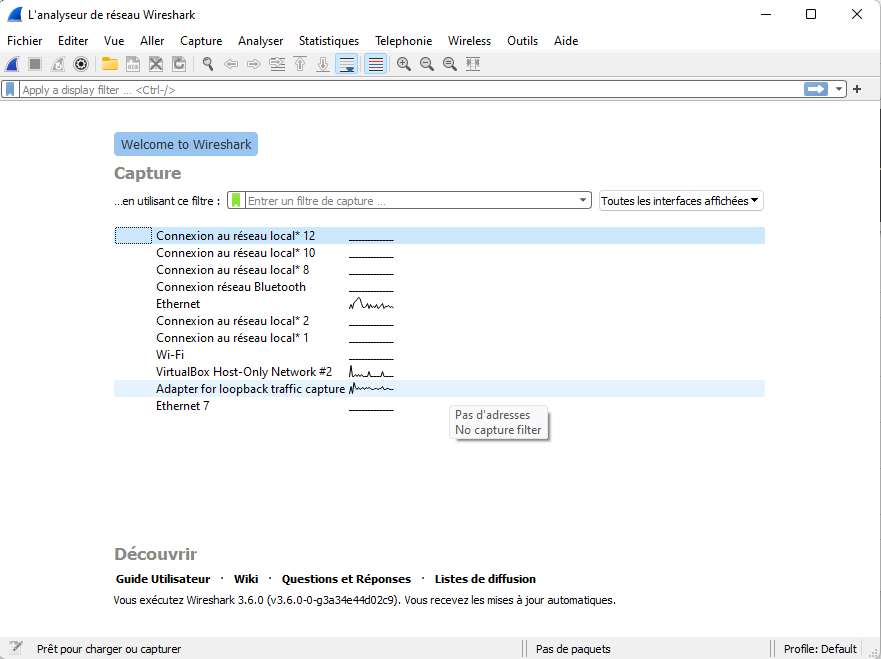
\includegraphics[width=1\columnwidth]{Pictures/wireshark-open.png}}
\caption{Ouverture de Wireshark}
\label{fig-wires-open}
\end{figure}


Il s'agit de déterminer quelle interface choisir. Ce n'est pas toujours facile car leurs noms ne sont pas toujours très explicites. Les petites courbes à gauche du nom indiquent le trafic instantané que Wireshark mesure. Sur le schéma, 3 interfaces sont actives : Ethernet, la communication avec une machine virtuelle et une interface appelée \textit{\Index{loopback}}.  La première permet d'avoir les communications avec l'extérieur et la dernière sera très utile lors des échanges entre deux processus dans cette machine.

\section {Capture}

En cliquant sur le nom de l'interface donnant accès au réseau exterieur (\index{Ethernet} dans notre cas), la fenêtre se découpe en 3 parties, comme le montre la figure~\vref{fig-wires-cap}.

\begin{figure}[tbp]
\centerline{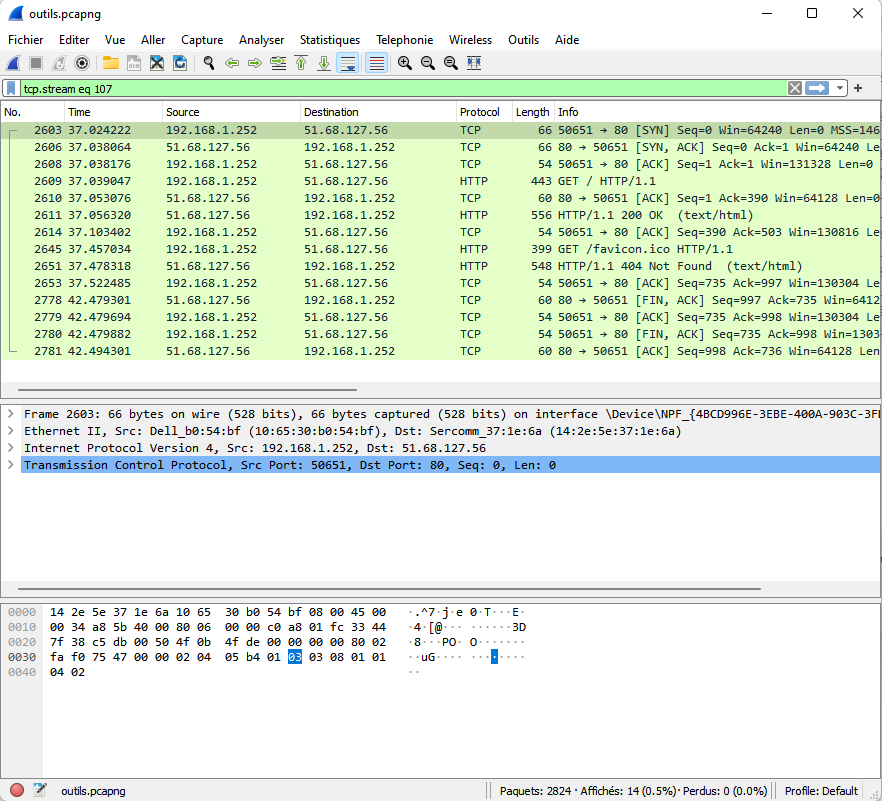
\includegraphics[width=1\columnwidth]{Pictures/ws-capture.png}}
\caption{Capture du trafic}
\label{fig-wires-cap}
\end{figure}

L'écran de Wireshark se divise en 3 parties :
\begin{itemize}
\item en haut, défile les trames qui sont capturées sur le réseau, chaque protocole à une couleur dédiée pour facilité le repérage~:
\begin{itemize}
\item le numéro de trame capturée, il s'agit d'une information ajoutée par Wireshark,
\item l'heure de capture de la trame. Cette information est aussi ajoutée par Wireshark,
\item l'adresse IP (IPv4 ou IPv6) de la machine à l'origine du paquet, 
\item l'adresse IP (IPv4 ou IPv6) de la machine destinataire du paquet,
\item le protocole de plus haut niveau contenu dans la trame. Dans notre cas, cela peut être TCP si le message TCP ne contient pas de données, comme lors de l'ouverture de connexion, ou de certains acquittements. On voit également les messages \ac{HTTP} qui sont bien entendu encapsulés dans TCP,
\item la taille en octets de la trame capturée par Wireshark,
\item finalement Wireshark fourni un résumé du contenu de la trame, pour comprendre ce qui se passe sur le réseau. Dans la capture, on retrouve pour les messages \ac{HTTP}, les requêtes GET ou les notifications ;
\end{itemize}
\item si une trame est sélectionnée dans la liste, elle apparaît dans la zone du milieu avec l'empilement protocolaire. Le contenu de chacun de ces protocoles peut être détaillé en cliquant sur le petit triangle à gauche ;
\item la fenêtre du bas donne l'équivalent en hexadécimal. Les parties surlignées correspondent aux champs sélectionnés dans la fenêtre du milieu. À noter que l'on retrouve l'information à la fois en hexadécimal et en caractère \ac{ASCII}, ce qui aide à la lecture quand on cherche une valeur spécifique.
\end{itemize}

\Question{Première colonne}
{Dans la première colonne~:
 \begin{itemize}[label=$\circ$]
   \item \Correct{Le numéro de la trame attribué par Wireshark à sa réception}
   \item \Wrong{Le numéro de la trame relevé directement dans la trame Ethernet}
  \end{itemize}
}
{
Ces numéros sont séquentiels, ils sont donc attribué localement par Wireshark. De plus il n'existe aucun champ de cette sorte dans Ethernet.
}
\Question{Deuxième colonne}
{Dans la deuxième colonne~:
 \begin{itemize}[label=$\circ$]
   \item \Correct{L'heure de réception par Wireshark}
   \item \Wrong{L'instant d'émission de la trame}
  \end{itemize}
}
{
Comme dans le cas précédent, ce numéro est ajouté par Wireshark, il n'existe pas de champ protocolaire indiquant l'instant d'émission.
}
\Question{Les troisième et quatrième colonnes}
{Dans les troisième et quatrième colonnes~:
 \begin{itemize}[label=$\circ$]
   \item \Wrong{les adresses Ethernet des machines.}
   \item \Wrong{Uniquement les adresses IPv4 des machines.}
   \item \Correct{Les adresses IPv4 ou IPv6 des machines.}
  \end{itemize}
}
{
Wireshark traite de la même manière les adresses IPv4 ou IPv6, elles sont donc affichées dans ces colonnes. L'adresse Ethernet (ou MAC) sur 48 bits n'est pas affichée par défaut dans cet écran.
}

\Question{La cinquième colonne}
{Dans la cinquième colonne~:
 \begin{itemize}[label=$\circ$]
   \item \Wrong{Le protocole applicatif (niveau 7).}
   \item \Correct{Le dernier (de plus haut niveau) protocole reconnu.}
   \item \Wrong{Le protocole de niveau 4 (ici TCP ou UDP).}
  \end{itemize}
}
{
Wireshark fournit l'information de plus haut niveau. Dans la figure~\vref{fig-wires-cap} certaines trames sont indiquées comme transportant le protocole HTTP, tandis que d'autres, généralement les acquittements sont indiqués comme étant de type TCP car elles ne transportent pas de données venant des couches supérieures.
}
\Question{La sixième colonne}
{Dans la sixième colonne~:
 \begin{itemize}[label=$\circ$]
   \item \Wrong{La taille en bits de la trame.}
   \item \Correct{La taille en octets de la trame.}
  \end{itemize}
}
{
L'unité est l'octet.
}
\Question{La septième colonne}
{Dans la septième colonne~:
 \begin{itemize}[label=$\circ$]
   \item \Correct{Un résumé des informations transportées par le protocole de plus haut niveau.}
   \item \Wrong{Les options d'IPv4.}
   \item \Wrong{le contenu en ASCII du message de plus haut niveau.}
  \end{itemize}
}
{
Wireshark cherche a interpréter les champs du protocole de plus haut niveau pour offrir un affichage synthétique de l'information.}
  \vspace{1em}

Cela fait beaucoup de trafic, nous allons limiter ce qui est affiché en ajoutant un filtre à un destinataire particulier. Le site \texttt{outils.plido.net} à l'adresse IPv4 \texttt{51.68.127.56}. Dans la fenêtre où il est indiqué \textit{Apply a display filter.} taper les instructions suivante: 

\begin{verbatim}
    ip.addr==51.68.127.56
\end{verbatim}

\noindent n'oubliez par le double \texttt{==} et la fenêtre doit devenir verte quand tout sera tapé indiquant que la syntaxe du filtre est correcte. En appuyant sur entrée, la fenêtre doit se vider.

\section{Analyse du trafic web}

Dans la barre d'adresse de votre navigateur préféré, taper l'URL suivante:

\begin{verbatim}
    http://outils.plido.net
\end{verbatim}

\noindent et la page Web indiqué figure~\vref{fig-firefox-hello} doit apparaître. 

\begin{figure}[tbp]
\centerline{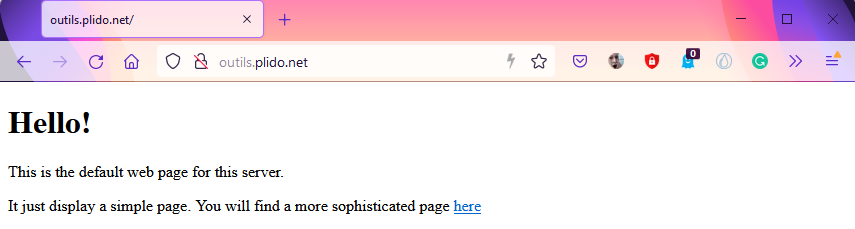
\includegraphics[width=1\columnwidth]{Pictures/firefox-simple.png}}
\caption{Afficher de la page par Firefox}
\label{fig-firefox-hello}
\end{figure}

  \vspace{1em}

Wireshark a permis de visualiser le trafic échangé entre l'ordinateur et le serveur Web. Le trafic doit être similaire a celui de la figure~\vref{fig-wires-cap}. La figure s'obtient en sélectionnant le menu \textit{Statistiques/Graphique de flux} et en cochant \textit{Limiter au Filtre d'Affichage}. Elle est un peu plus lisible car elle représente les échanges sous forme de chronographes.

\begin{figure}[tbp]
\centerline{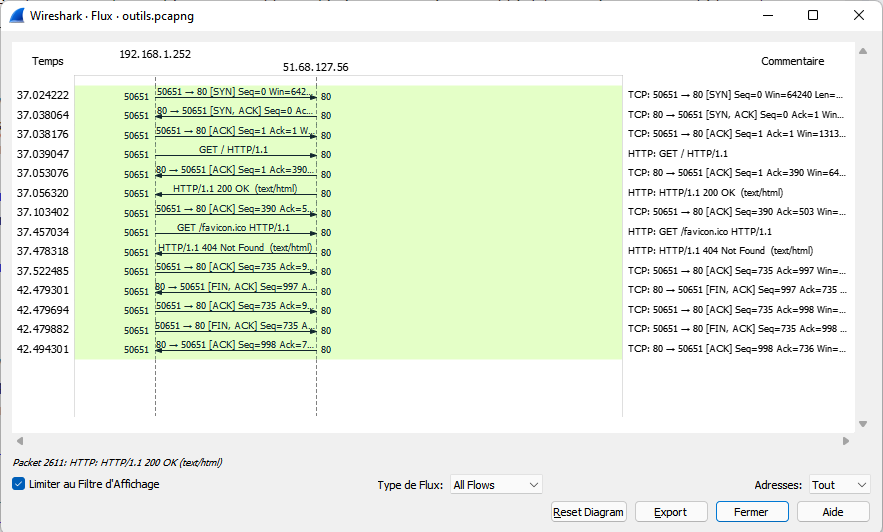
\includegraphics[width=1\columnwidth]{Pictures/ws-filtre.png}}
\caption{Afficher de la page par Firefox}
\label{fig-ws-filtre}
\end{figure}

Trois phases peuvent être distinguées~:
\begin{itemize}
    \item L'ouverture de connexion TCP avec l'émission de trois messages TCP;
    \item la phase de transfert de données~:
    \begin{itemize}
        \item le client envoie une requête HTTP GET au serveur pour demander la ressource à la racine (\texttt{/}),
        \item le serveur acquitte le message au niveau TCP pour indiquer qu'il a bien été reçu.
        \item le serveur envoie la réponse à la requête précédente et précisant le statut (\textttt{200 : OK}) et le que contenu est formaté en HTML.
        \item le client acquitte ce message au niveau TCP
        \item le client envoie une nouvelle requête HTTP GET pour obtenir la ressource \texttt{/facicon.ico}
        \item le serveur répond que la ressource n'existe pas (\texttt{404 : Not Found}). Cette requête acquitte implicitement le message précédent.
        \item le client acquitte la réponse du serveur au niveau TCP.
    \end{itemize}
    \item le serveur termine la connexion après 5 secondes d'inactivité. La fermeture se fait en échangeant 4 messages TCP.
\end{itemize}
